\documentclass[a4paper, 14pt]{extarticle}

%--------------------------------------
%               Пакеты
%--------------------------------------
\usepackage{geometry}
\geometry{a4paper,tmargin=2cm,bmargin=2cm,lmargin=3cm,rmargin=1cm}

\usepackage[T2A]{fontenc}
\usepackage[utf8]{inputenc}
\usepackage[english, main=russian]{babel}

\usepackage{textcomp}
\usepackage{indentfirst}
\usepackage{graphicx}
\graphicspath{{./images/}}
\usepackage{enumitem}
\usepackage{caption}
\usepackage{hyperref}
\hypersetup{unicode=true}

\DeclareCaptionLabelSeparator*{emdash}{~--- }
\captionsetup[figure]{labelsep=emdash,font=onehalfspacing,position=bottom}

\usepackage{tempora}
\usepackage{amsmath}
\usepackage{color}
\usepackage{listings}

\lstset{
  belowcaptionskip=1\baselineskip,
  breaklines=true,
  frame=L,
  xleftmargin=\parindent,
  language=C++,
  showstringspaces=false,
  basicstyle=\footnotesize\ttfamily,
  keywordstyle=\bfseries\color{blue},
  commentstyle=\itshape\color{purple},
  identifierstyle=\color{black},
  stringstyle=\color{red},
  numbers=left,
  numberstyle=\tiny,
  stepnumber=1,
  numbersep=5pt
}

\linespread{1.3}
\sloppy
\clubpenalty=10000
\widowpenalty=10000

%--------------------------------------
%               Документ
%--------------------------------------
\begin{document}

%--------------------------------------
%           Титульный лист
%--------------------------------------
\begin{titlepage}
\thispagestyle{empty}

\vspace*{-60pt}
\begin{center}

\includegraphics[width=0.35\textwidth]{emblem}
\end{center}

\vspace{-25pt}
\hrule height2.3pt
\vspace*{-20.3pt}
\hrule

\vspace{4ex}
\begin{center}
  \small
  Министерство науки и высшего образования Российской Федерации\\
  Федеральное государственное бюджетное образовательное учреждение высшего образования\\
  «Московский государственный технический университет имени Н.\,Э.~Баумана\\
  (национальный исследовательский университет)»
\end{center}

\vspace{11em}
\begin{center}
  \Large\bfseries Лабораторная работа №\,12\\[1ex]
  \large «Обработка текстовых файлов»
\end{center}

\vspace{8em}
\begin{flushright}
  Студент группы ИУ9-21Б \textbf{Хромов М.\,А.}\\[2ex]
  Преподаватель \textbf{Посевин Д.\,П.}
\end{flushright}

\vfill
\begin{center}
  \textsl{Москва 2025}
\end{center}
\end{titlepage}

%--------------------------------------
\section{Задание}\label{sect:task}
Варианты заданий для программ, которые нужно разработать,
приведены в таблицах 1–7.  
Каждая программа должна принимать через аргумент командной строки
\textbf{путь к каталогу} с подлежащими обработке файлами.

%--------------------------------------
\section{Индивидуальные варианты}\label{sect:variant}

\begin{description}[leftmargin=0pt]
  \item[Вариант A.] Найти все файлы с расширением \texttt{.txt} в указанном каталоге,
        перемешать случайным образом буквы \emph{в середине} каждого слова
        (первая и последняя буквы остаются на месте) и сохранить результат
        под тем же именем в \emph{текущем} каталоге.
        Проверку выполнить на англоязычных текстах.
  \item[Вариант B.] Найти все файлы с расширением \texttt{.c} в указанном каталоге,
        удалить из каждого файла \emph{комментарии} и сохранить
        очищенный текст под тем же именем в текущем каталоге.
        Проверку выполнить на наборе исходников на C
        (например, фрагменты ядра Linux).
\end{description}

%--------------------------------------
\section{Код программ}\label{sect:listings}
Ниже приведены исходные тексты.  
Каждый листинг, превышающий 70 строк, разбит на две части.
После каждого листинга — команда \verb|\clearpage|.

%----------  Листинг 1-а  ----------
\begin{figure}[!htb]
\begin{lstlisting}[caption={\texttt{strip\_comments.cpp}, строки 1–70},label={lst:strip-a},firstnumber=1,lastline=70]
#include <iostream>
#include <fstream>
#include <sstream>
#include <string>
#include <dirent.h>
#include <sys/stat.h>

using namespace std;

// Удаление C-комментариев
string stripComments(const string& src) {
    string out;
    enum State { NORMAL, SLASH, LINE_C, BLOCK_C, BLOCK_STAR } st = NORMAL;
    for (size_t i = 0; i < src.size(); ++i) {
        char c = src[i];
        switch (st) {
            case NORMAL:
                if (c == '/') st = SLASH;
                else out += c;
                break;
            case SLASH:
                if (c == '/')       st = LINE_C;
                else if (c == '*')  st = BLOCK_C;
                else { out += '/'; out += c; st = NORMAL; }
                break;
            case LINE_C:
                if (c == '\n') { out += '\n'; st = NORMAL; }
                break;
            case BLOCK_C:
                if (c == '*') st = BLOCK_STAR;
                break;
            case BLOCK_STAR:
                if (c == '/')      st = NORMAL;
                else if (c != '*') st = BLOCK_C;
                break;
        }
    }
    if (st == SLASH) out += '/';
    return out;
}

bool isCFile(const string& name) {
    return name.size() > 2 && name.substr(name.size() - 2) == ".c";
}

int main(int argc, char* argv[]) {
    string folder = argv[1];
    DIR* dir = opendir(folder.c_str());
    if (!dir) {
        cerr << "Не удалось открыть каталог " << folder << endl;
        return 1;
    }
    dirent* entry;
    while ((entry = readdir(dir)) != nullptr) {
        string name = entry->d_name;
        if (!isCFile(name)) continue;
        string inPath = folder + "/" + name;
        ifstream in(inPath);
        if (!in.is_open()) { cerr << "Ошибка: " << inPath << endl; continue; }
\end{lstlisting}
\end{figure}
\clearpage

%----------  Листинг 1-б  ----------
\begin{figure}[!htb]
\begin{lstlisting}[caption={\texttt{strip\_comments.cpp}, остаток},label={lst:strip-b},firstnumber=71]
        string outPath = "cleaned_files/" + name;
        ofstream out(outPath);
        if (!out.is_open()) {
            cerr << "Ошибка: " << outPath << endl;
            in.close();
            continue;
        }
        stringstream ss; ss << in.rdbuf();
        out << stripComments(ss.str());
        in.close();  out.close();
    }
    closedir(dir);
    return 0;
}

/* запуск:
   ./lab12_strip_comments /path/to/c_sources
*/
\end{lstlisting}
\end{figure}
\clearpage

%----------  Листинг 2-а  ----------
\begin{figure}[!htb]
\begin{lstlisting}[caption={\texttt{shuffle\_words.cpp}, строки 1–70},label={lst:shuffle-a},firstnumber=1,lastline=70]
#include <iostream>
#include <fstream>
#include <string>
#include <sstream>
#include <dirent.h>
#include <algorithm>
#include <random>
#include <cctype>

using namespace std;

// Перемешивание средней части слова
string shuffleMiddle(string word) {
    if (word.length() <= 3) return word;

    string prefix="", suffix="";
    while (!word.empty() && !isalnum(word.front())) {
        prefix += word.front();
        word.erase(word.begin());
    }
    while (!word.empty() && !isalnum(word.back())) {
        suffix  = word.back() + suffix;
        word.pop_back();
    }
    if (word.length() <= 3) return prefix + word + suffix;

    string middle = word.substr(1, word.length()-2);
    static random_device rd; static mt19937 g(rd());
    shuffle(middle.begin(), middle.end(), g);

    return prefix + word.front() + middle + word.back() + suffix;
}

bool isTxtFile(const string& name) {
    return name.size() > 4 && name.substr(name.size()-4) == ".txt";
}

void printFile(const string& fname) {
    ifstream f(fname);
    if (!f.is_open()) { cerr << "Ошибка открытия " << fname << endl; return; }
    cout << "\n" << fname << " (результат)\n";
    string line; while (getline(f,line)) cout << line << '\n';
    f.close();
}

int main(int argc, char* argv[]) {
    string folder = argv[1];
    DIR* dir = opendir(folder.c_str());
    if (!dir) { cerr << "Каталог не открыть: " << folder << endl; return 1; }

    dirent* entry;
    while ((entry = readdir(dir)) != nullptr) {
        string file = entry->d_name;
        if (!isTxtFile(file)) continue;
        string inPath = folder + "/" + file;
        ifstream in(inPath);
\end{lstlisting}
\end{figure}
\clearpage

%----------  Листинг 2-б  ----------
\begin{figure}[!htb]
\begin{lstlisting}[caption={\texttt{shuffle\_words.cpp}, остаток},label={lst:shuffle-b},firstnumber=71]
        ofstream out(file);
        if (!in.is_open() || !out.is_open()) {
            cerr << "Ошибка файла: " << file << endl;
            continue;
        }
        string line;
        while (getline(in,line)) {
            istringstream iss(line);
            string word;
            while (iss >> word) out << shuffleMiddle(word) << ' ';
            out << '\n';
        }
        in.close(); out.close();
        printFile(file);
    }
    closedir(dir);
    return 0;
}

/* запуск:
   ./lab12_shuffle /path/to/texts
*/
\end{lstlisting}
\end{figure}
\clearpage

%--------------------------------------
\section{Результаты работы}
\begin{center}
  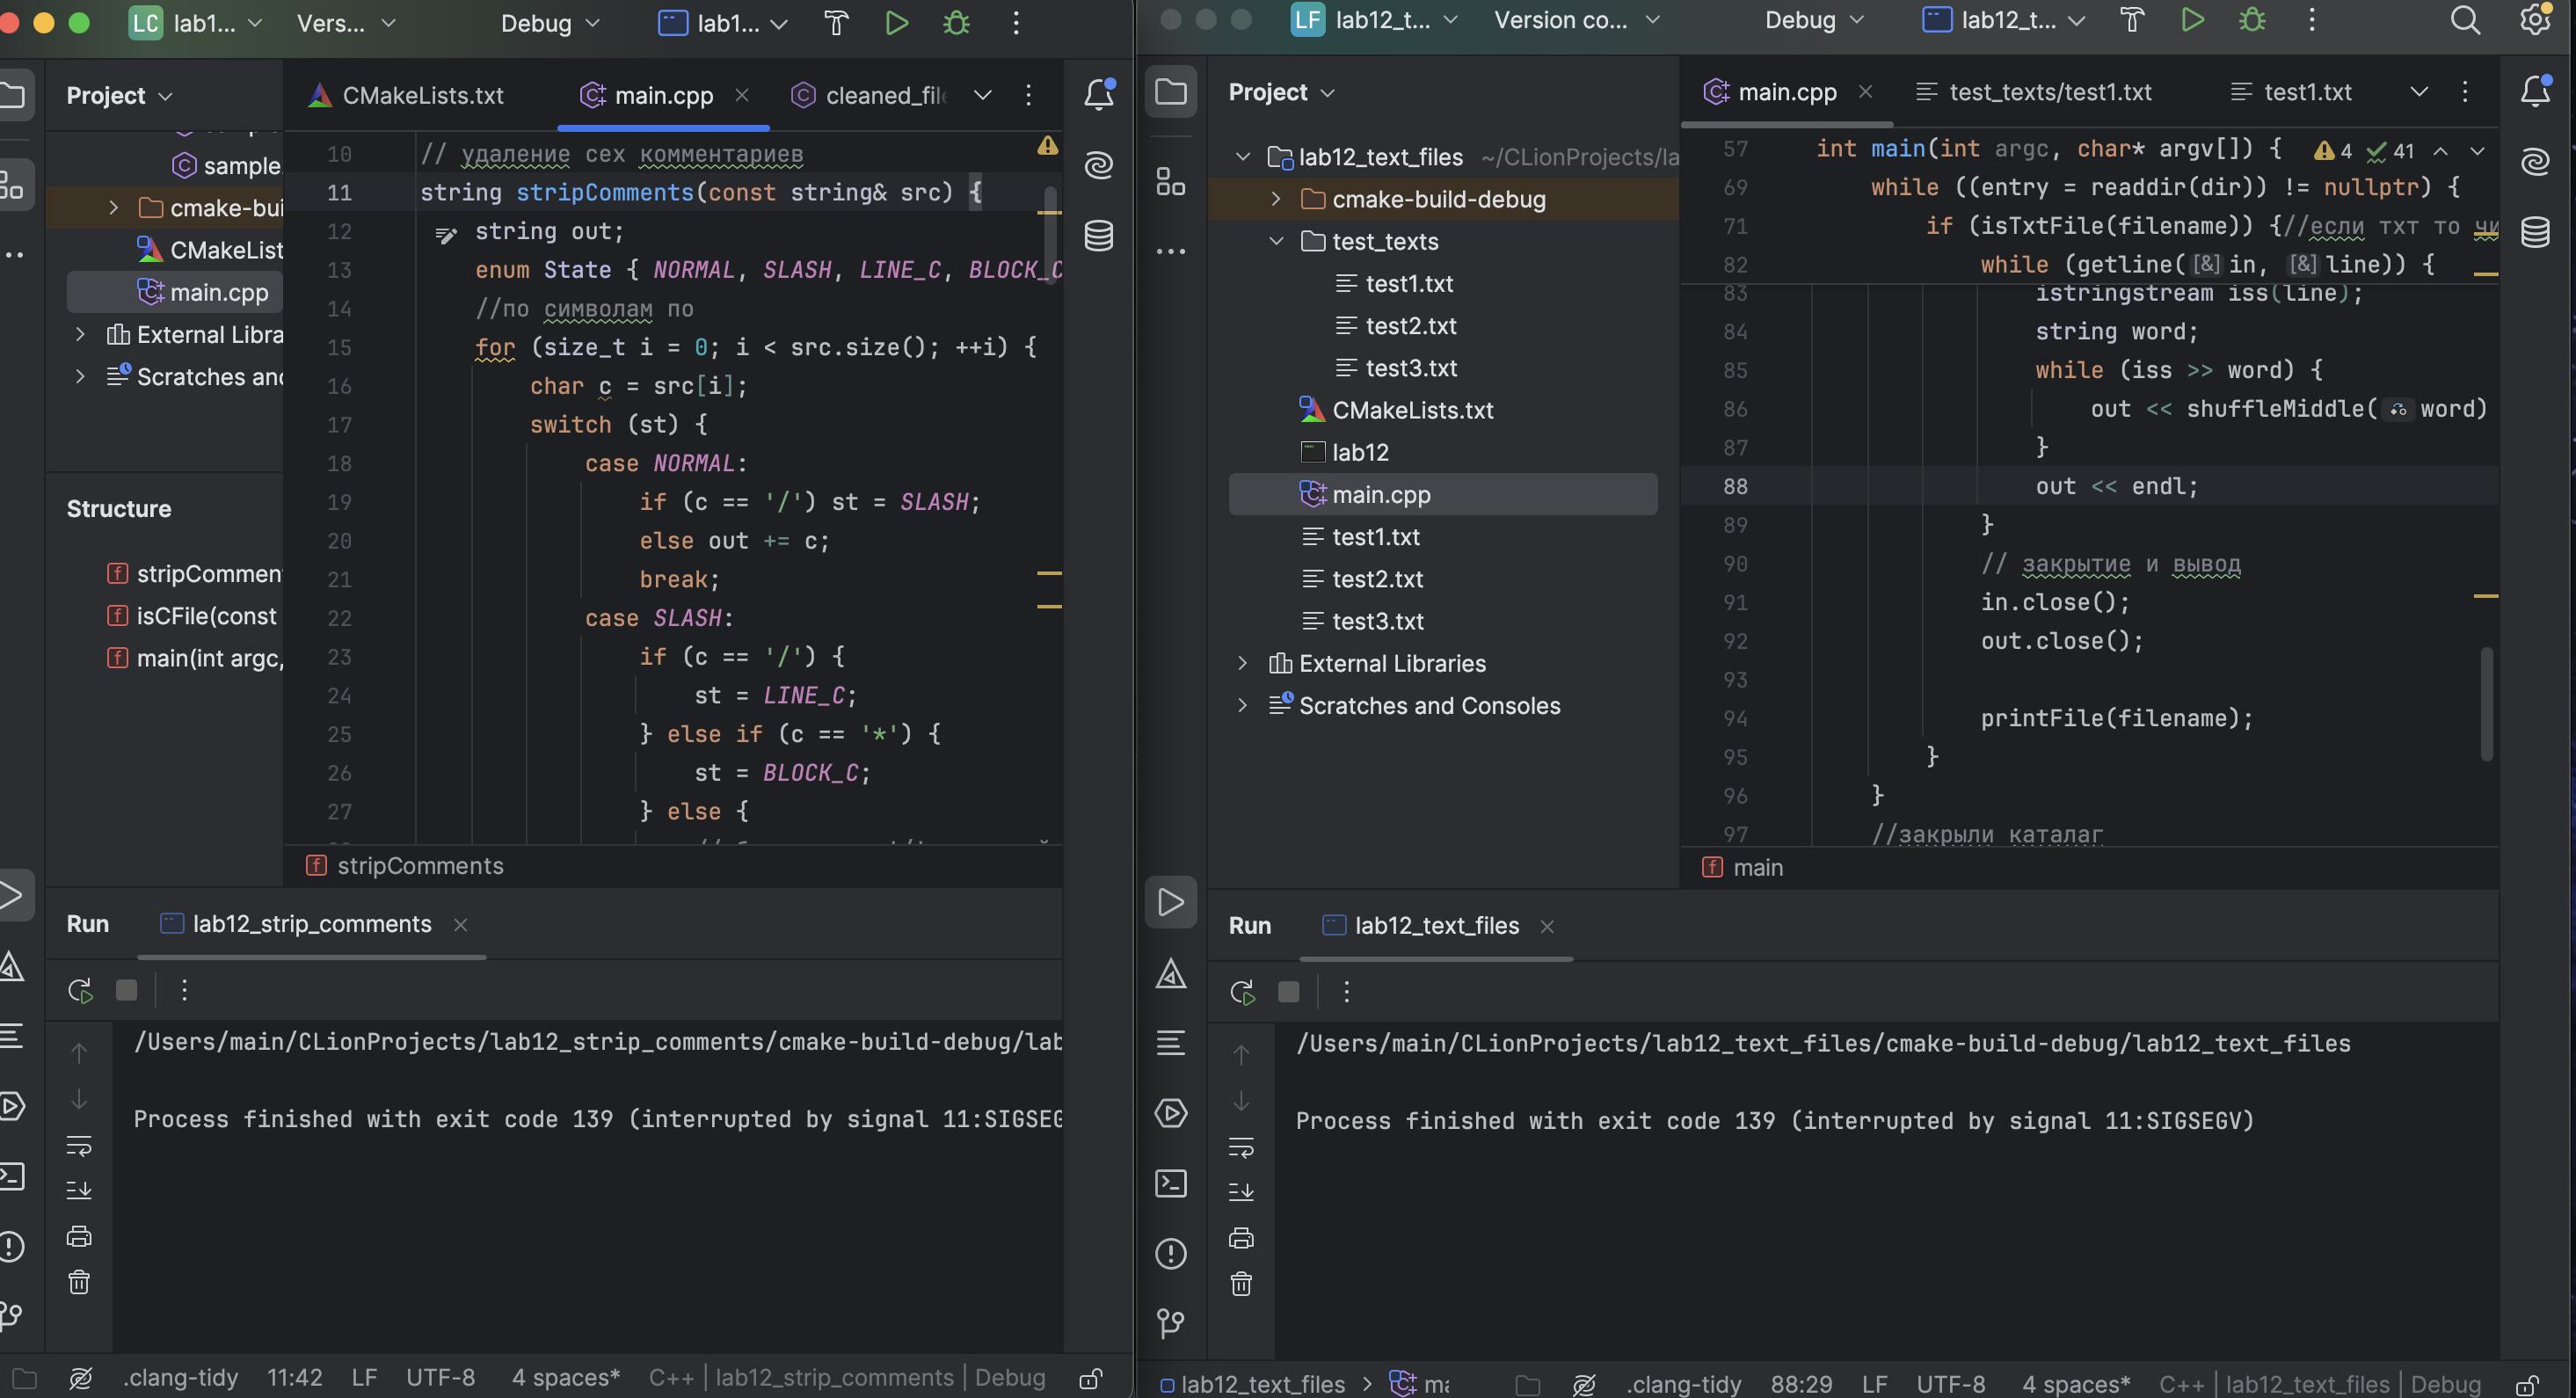
\includegraphics[width=0.8\textwidth]{фото25.jpeg}
  \captionof{figure}{Фрагменты консольного вывода и содержимого файлов после обработки}
\end{center}

%--------------------------------------
\section{Вывод}
В рамках лабораторной работы № 12 разработаны две утилиты
обработки файловой коллекции:

\begin{itemize}[nosep]
  \item \textbf{strip\_comments}: рекурсивно сканирует указанный каталог,
        выбирает файлы \texttt{.c}, удаляет из них как строчные,
        так и блочные комментарии и сохраняет чистые исходники
        в подкаталоге \texttt{cleaned\_files}.
  \item \textbf{shuffle\_words}: для каждого \texttt{.txt}-файла
        перемешивает символы внутри слов, сохраняя читаемость
        благодаря неизменным первым и последним буквам.
\end{itemize}

Обе программы принимают путь к каталогу через параметр командной строки,
демонстрируют работу с API POSIX для обхода директорий,
потоковый ввод-вывод и базовые алгоритмы обработки строк.
\end{document}
